\documentclass{beamer}

\usetheme[secheader]{Boadilla}
\usecolortheme{seahorse}
\usepackage[spanish]{babel} 		% {Con estos dos anda
\usepackage[utf8]{inputenc} 		% todo lo que es tildes y ñ}
\usepackage{graphicx}

\title{Towards Verifying Android Apps for the Absence of No-Sleep Energy Bugs}
\author{Martín Carreiro - Pablo Rago - Juan Manuel Tastzian}
\date{21 de Mayo de 2014}
\institute[2014]{Facultad de Ciencias Exactas y Naturales}

\begin{document}

\frame{\titlepage}

\section[Temas a desarrollar]{}
\frame{\tableofcontents}

\section{Introducción}

\frame {
	\frametitle{Ventajas de los smartphones actuales}
	Muchas características al alcance de la mano:
	\begin{itemize}
		\item<1-> Procesadores rápidos
		\item<2-> Pantallas grandes
		\item<3-> Cámara, GPS, 3G, Wifi...
	\end{itemize}
}

\frame {
	\frametitle{¿Y antes?}
	\begin{itemize}
		\item[] <1-> Pero...
		\item[] <2-> ...¿se acuerdan del pasado?
	\end{itemize}
}

\frame {
	\frametitle{¡LEYENDA!}
	\begin{center}
		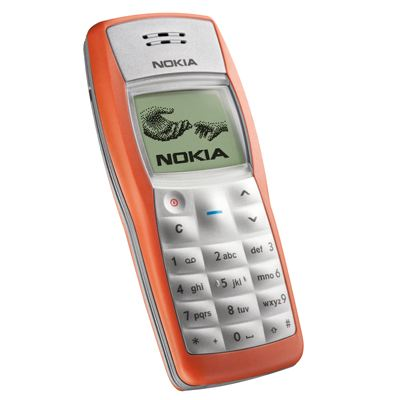
\includegraphics[scale=0.5]{./imgs/nokia1100.jpg}	
	\end{center}
}

\frame {
	\frametitle{¿Cuánto les duraba la batería del Nokia 1100 y similares?}
	\begin{itemize}
		\item<1-> ¿15 hs?
		\item<2-> ¿2 días?
		\item<3-> Como 4 o 5, tranqui!
	\end{itemize}
}

\frame{
	\frametitle{Eso ya no pasa con los Smartphones}
	\begin{itemize}
		\item[] <1-> Lamentablemente, todas las ventajas mencionadas antes necesitan mucha energía para funcionar.
		\item[] <2-> Y por eso, la batería de nuestros celulares de hoy dura entre 12 y 16 horas, promedio, siendo unas 18 o 20 horas una excelente duración de batería (ni hablar de más tiempo).
	\end{itemize}
}

\section{Manejo de energía en Android}

%\subsection{Wakelock API}

\frame {
	\frametitle{Manejo de energía en Android}
	\begin{itemize}
		\item[] <1-> ¿Cómo maneja la energía Android?
		\begin{itemize}
			\item<2-> De manera agresiva
		\end{itemize}
		\item[] <3-> ¿Le pega para que se porte bien?
		\begin{itemize}
			\item<4-> No tan agresiva, pero le corta el chorro a todo en el momento inmediato en el que se deja de usar.
		\end{itemize}
	\end{itemize}
}

\frame {
	\frametitle{Manejo de energía en Android}
	\begin{itemize}
		\item[] <1-> Pero, ¿y si quiero tener el procesador corriendo para recibir algún update o notificación?
		\begin{itemize}
			\item<2-> Ahí es donde entra en juego la \textbf{Wakelock API}.		
		\end{itemize}
	\end{itemize}
}

\frame {
	\frametitle {Wakelock API}
	\begin{itemize}
		\item[] <1-> Lamentablemente, la complejidad del sistema operativo y los errores que pueden cometer los desarrolladores hacen que el uso inapropiado de Wakelocks se manifiesten como no-sleep-bugs.
		\item[] <2-> Los autores del paper decidieron intentar mitigar el problema implementando una herramienta que verifica la ausencia de estos bugs con respecto a una serie de políticas específicas sobre los Wakelocks, utilizando un framework de flujo de datos para analizar las aplicaciones.
	\end{itemize}
}

\frame {
	\frametitle {Wakelock API}
	\begin{itemize}
		\item[] <1-> Permite a los desarrolladores dar directivas específicas sobre los recursos al sistema operativo.
		\item[] <2-> Android pone todo en sleep mode ni bien se ponen en estado idle (reposo).
	\end{itemize}
}

%{
%	This text will stay on all pages.
%	\only<1>{
%		\begin{itemize}
%			\item<1->This will only appear on the first page
%			\item<1->This is also only for the first page
%		\end{itemize}
%	}
%	\only<2>{
%		\begin{itemize}
%			\item<2->This will only appear on the second page
%		\item<2->This is also only for the second page
%		\end{itemize}
%      }
%}
%
%\subsection{Second Sub Section}
%
%\frame {
%	\frametitle{Last Frame}
%	This is the last frame
%}

\end{document}